\begin{flushleft}
    \fontsize{16}{20}\selectfont
    \section*{CHƯƠNG 2: PHÂN TÍCH THỰC TRẠNG CỦA VẤN ĐỀ CÓ LIÊN QUAN ĐẾN
    ĐỀ TÀI MÀ SINH VIÊN CHỌN VIẾT BÁO CÁO THỰC TẬP TẠI DOANH NGHIỆP THỰC TẬP}
    \addcontentsline{toc}{section}{CHƯƠNG 2: PHÂN TÍCH THỰC TRẠNG CỦA VẤN ĐỀ CÓ LIÊN QUAN ĐẾN
    ĐỀ TÀI MÀ SINH VIÊN CHỌN VIẾT BÁO CÁO THỰC TẬP TẠI DOANH NGHIỆP THỰC TẬP}
    \fontsize{13}{20}\selectfont
    \paragraph{}
    \fontsize{13}{20}\selectfont Trong quá trình thực tập tại công ty, em đã được giao dự án về phát triển phần mềm sử dụng YOLO và OpenCV để xác định và đưa ra cảnh báo đối với các đối tượng là con người trong một khu vực cụ thể.\\
    \setcounter{section}{2}
    \setcounter{subsection}{0}
    \subsection{Vấn Đề Đặt Ra}
    \fontsize{13}{20}\selectfont Vấn đề được đặt ra là phải làm sao để có thể xác định được chủ thể con người trong camera (Camera an ninh, điện thoại,...) và xác nhận xem chủ thể có ở trong khu vực được đánh dấu là an toàn hay không, vấn đề này có thể được áp dụng vào các tình huống trong đời sống hàng ngày cũng như trong doanh nghiệp, sản xuất:\\ 
    \begin{itemize}
        \item Trong gia đình: \\
        Bài toán này có thể giúp phụ huynh có thể trông con em mình, ví dụ như thông qua camera giám sát và các điểm thiết lập đã được cài đặt sẵn,phụ huynh có thể giám sát được xem là trẻ có đang trong khu vực an toàn hay không,...
        \begin{figure}[htbp]
            \centering
            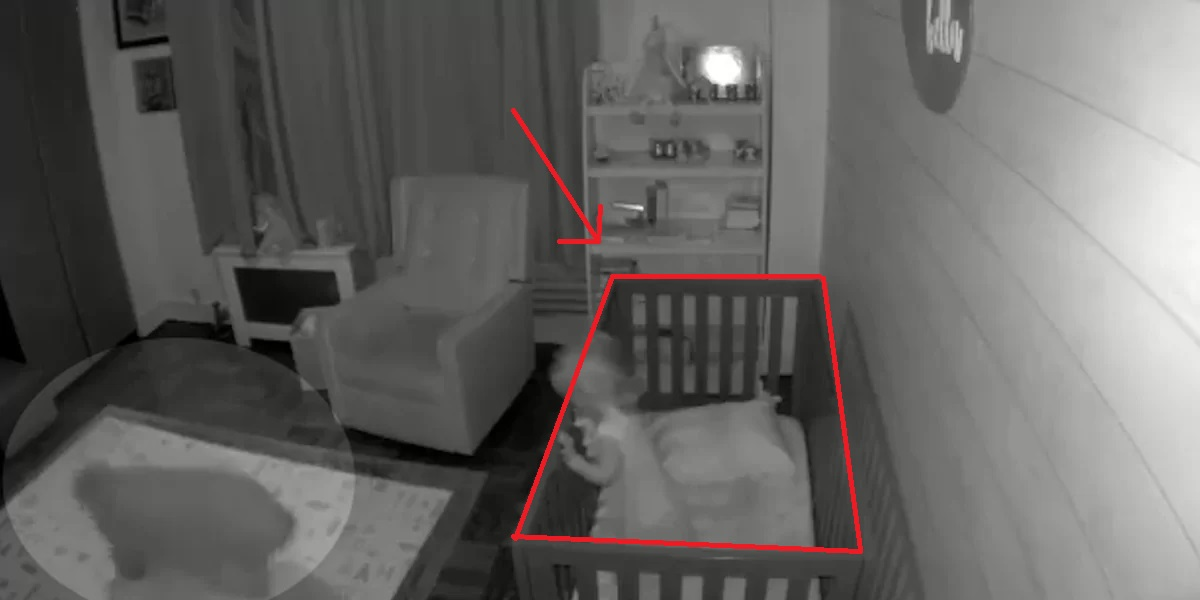
\includegraphics[width=0.5\textwidth]{images/TH1.jpg}
            \caption{Trong trường hợp gia đình.}
            \label{fig:img_1_GD}
        \end{figure}
        \item Trong văn phòng:\\
        Trong văn phòng, có thể giám sát xem, nhân viên có đang làm việc trong khu vực chỉ định hay không,...
        \begin{figure}[htbp]
            \centering
            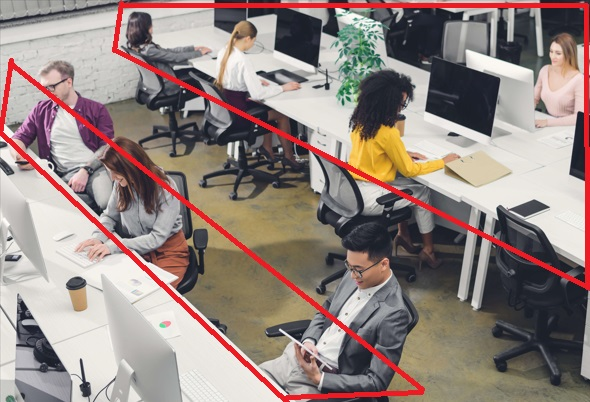
\includegraphics[width=0.5\textwidth]{images/TH2.jpg}
            \caption{Trong trường hợp văn phòng.}
            \label{fig:img_2_VP}
        \end{figure}
        \item Trong sản xuất:\\
        Trong sản xuất, việc các công nhân có làm đúng được vị trí của mình được phân công hay không,...
        \begin{figure}[htbp]
            \centering
            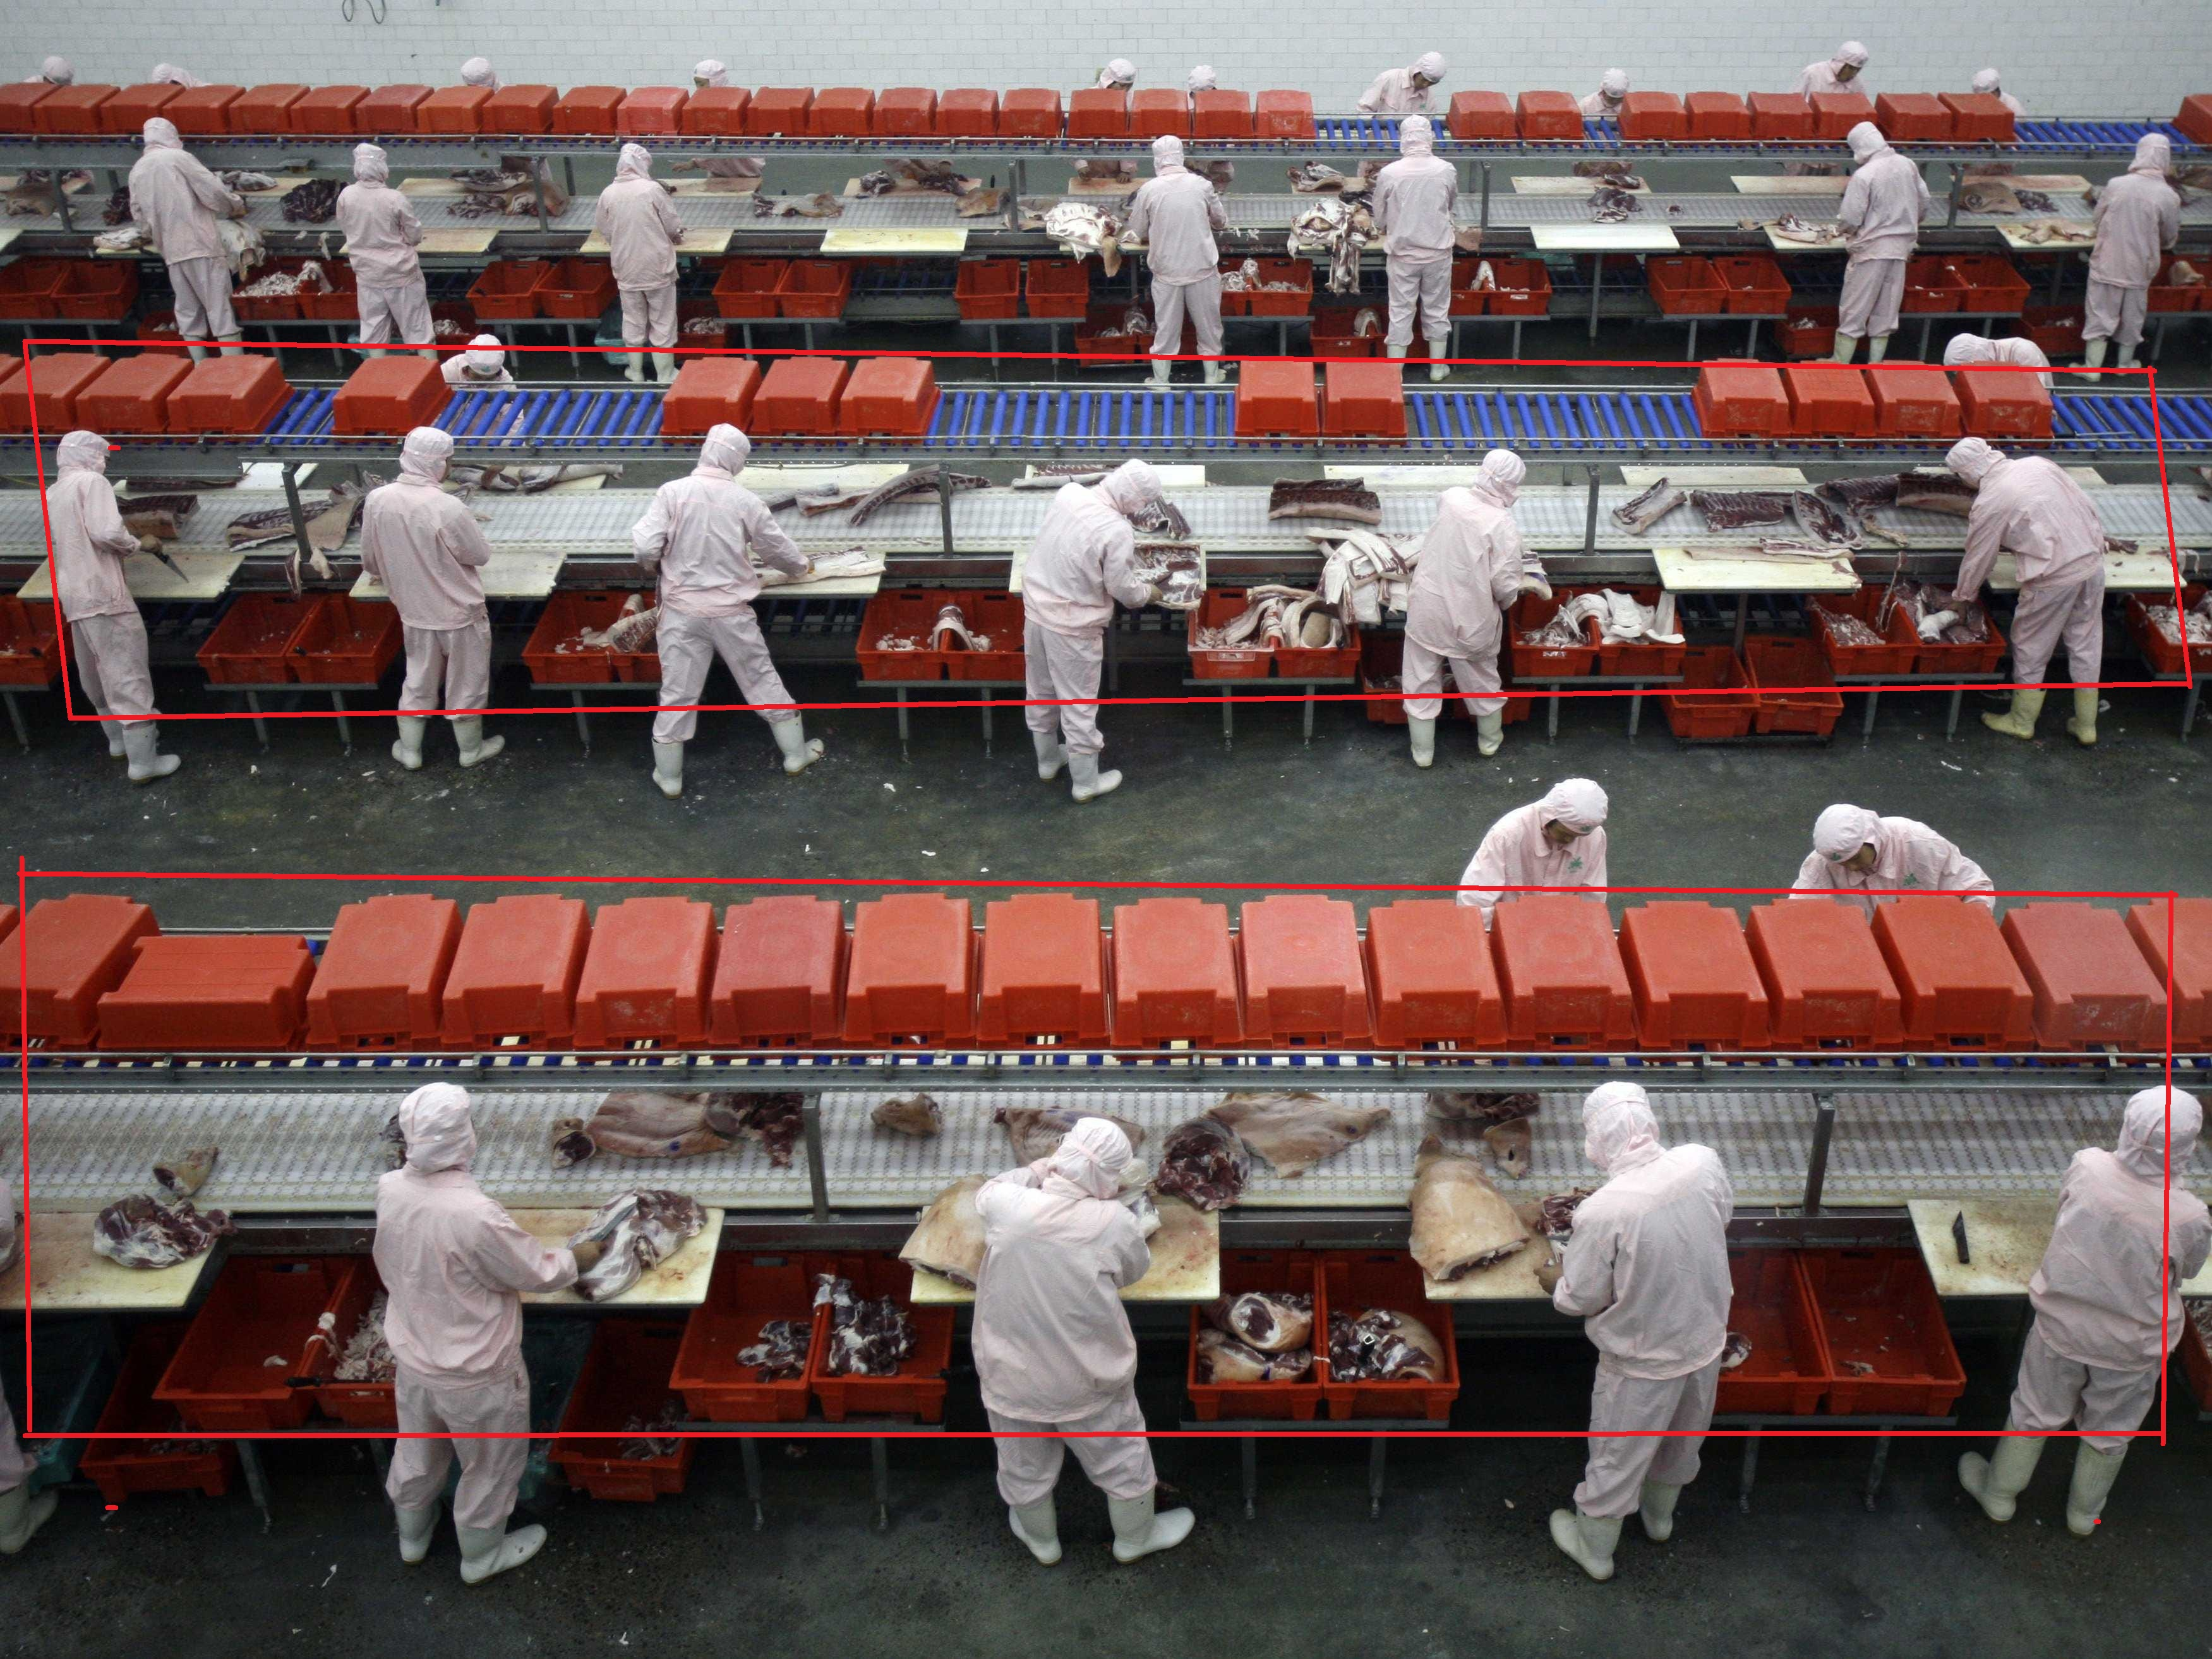
\includegraphics[width=0.5\textwidth]{images/TH3.jpg}
            \caption{Trong trường hợp xí nghiệp.}
            \label{fig:img_3_XN}
        \end{figure}
    \end{itemize}
    

    
    \subsection{Giải Pháp}
    \fontsize{13}{13}\selectfont\paragraph{}
    Để giải quyết các vấn đề trên, mô hình nhận diện đối tượng YOLO và bộ OpenCV được úng dụng vào giải pháp theo dõi con người và đánh giá an toàn. \\
    
\end{flushleft}